% Options for packages loaded elsewhere
\PassOptionsToPackage{unicode}{hyperref}
\PassOptionsToPackage{hyphens}{url}
%
\documentclass[
]{book}
\usepackage{lmodern}
\usepackage{amssymb,amsmath}
\usepackage{ifxetex,ifluatex}
\ifnum 0\ifxetex 1\fi\ifluatex 1\fi=0 % if pdftex
  \usepackage[T1]{fontenc}
  \usepackage[utf8]{inputenc}
  \usepackage{textcomp} % provide euro and other symbols
\else % if luatex or xetex
  \usepackage{unicode-math}
  \defaultfontfeatures{Scale=MatchLowercase}
  \defaultfontfeatures[\rmfamily]{Ligatures=TeX,Scale=1}
\fi
% Use upquote if available, for straight quotes in verbatim environments
\IfFileExists{upquote.sty}{\usepackage{upquote}}{}
\IfFileExists{microtype.sty}{% use microtype if available
  \usepackage[]{microtype}
  \UseMicrotypeSet[protrusion]{basicmath} % disable protrusion for tt fonts
}{}
\makeatletter
\@ifundefined{KOMAClassName}{% if non-KOMA class
  \IfFileExists{parskip.sty}{%
    \usepackage{parskip}
  }{% else
    \setlength{\parindent}{0pt}
    \setlength{\parskip}{6pt plus 2pt minus 1pt}}
}{% if KOMA class
  \KOMAoptions{parskip=half}}
\makeatother
\usepackage{xcolor}
\IfFileExists{xurl.sty}{\usepackage{xurl}}{} % add URL line breaks if available
\IfFileExists{bookmark.sty}{\usepackage{bookmark}}{\usepackage{hyperref}}
\hypersetup{
  pdftitle={Analyse multidimensionnelle appliquée},
  pdfauthor={Denis Larocque, Léo Belzile},
  hidelinks,
  pdfcreator={LaTeX via pandoc}}
\urlstyle{same} % disable monospaced font for URLs
\usepackage{color}
\usepackage{fancyvrb}
\newcommand{\VerbBar}{|}
\newcommand{\VERB}{\Verb[commandchars=\\\{\}]}
\DefineVerbatimEnvironment{Highlighting}{Verbatim}{commandchars=\\\{\}}
% Add ',fontsize=\small' for more characters per line
\usepackage{framed}
\definecolor{shadecolor}{RGB}{248,248,248}
\newenvironment{Shaded}{\begin{snugshade}}{\end{snugshade}}
\newcommand{\AlertTok}[1]{\textcolor[rgb]{0.94,0.16,0.16}{#1}}
\newcommand{\AnnotationTok}[1]{\textcolor[rgb]{0.56,0.35,0.01}{\textbf{\textit{#1}}}}
\newcommand{\AttributeTok}[1]{\textcolor[rgb]{0.77,0.63,0.00}{#1}}
\newcommand{\BaseNTok}[1]{\textcolor[rgb]{0.00,0.00,0.81}{#1}}
\newcommand{\BuiltInTok}[1]{#1}
\newcommand{\CharTok}[1]{\textcolor[rgb]{0.31,0.60,0.02}{#1}}
\newcommand{\CommentTok}[1]{\textcolor[rgb]{0.56,0.35,0.01}{\textit{#1}}}
\newcommand{\CommentVarTok}[1]{\textcolor[rgb]{0.56,0.35,0.01}{\textbf{\textit{#1}}}}
\newcommand{\ConstantTok}[1]{\textcolor[rgb]{0.00,0.00,0.00}{#1}}
\newcommand{\ControlFlowTok}[1]{\textcolor[rgb]{0.13,0.29,0.53}{\textbf{#1}}}
\newcommand{\DataTypeTok}[1]{\textcolor[rgb]{0.13,0.29,0.53}{#1}}
\newcommand{\DecValTok}[1]{\textcolor[rgb]{0.00,0.00,0.81}{#1}}
\newcommand{\DocumentationTok}[1]{\textcolor[rgb]{0.56,0.35,0.01}{\textbf{\textit{#1}}}}
\newcommand{\ErrorTok}[1]{\textcolor[rgb]{0.64,0.00,0.00}{\textbf{#1}}}
\newcommand{\ExtensionTok}[1]{#1}
\newcommand{\FloatTok}[1]{\textcolor[rgb]{0.00,0.00,0.81}{#1}}
\newcommand{\FunctionTok}[1]{\textcolor[rgb]{0.00,0.00,0.00}{#1}}
\newcommand{\ImportTok}[1]{#1}
\newcommand{\InformationTok}[1]{\textcolor[rgb]{0.56,0.35,0.01}{\textbf{\textit{#1}}}}
\newcommand{\KeywordTok}[1]{\textcolor[rgb]{0.13,0.29,0.53}{\textbf{#1}}}
\newcommand{\NormalTok}[1]{#1}
\newcommand{\OperatorTok}[1]{\textcolor[rgb]{0.81,0.36,0.00}{\textbf{#1}}}
\newcommand{\OtherTok}[1]{\textcolor[rgb]{0.56,0.35,0.01}{#1}}
\newcommand{\PreprocessorTok}[1]{\textcolor[rgb]{0.56,0.35,0.01}{\textit{#1}}}
\newcommand{\RegionMarkerTok}[1]{#1}
\newcommand{\SpecialCharTok}[1]{\textcolor[rgb]{0.00,0.00,0.00}{#1}}
\newcommand{\SpecialStringTok}[1]{\textcolor[rgb]{0.31,0.60,0.02}{#1}}
\newcommand{\StringTok}[1]{\textcolor[rgb]{0.31,0.60,0.02}{#1}}
\newcommand{\VariableTok}[1]{\textcolor[rgb]{0.00,0.00,0.00}{#1}}
\newcommand{\VerbatimStringTok}[1]{\textcolor[rgb]{0.31,0.60,0.02}{#1}}
\newcommand{\WarningTok}[1]{\textcolor[rgb]{0.56,0.35,0.01}{\textbf{\textit{#1}}}}
\usepackage{longtable,booktabs}
% Correct order of tables after \paragraph or \subparagraph
\usepackage{etoolbox}
\makeatletter
\patchcmd\longtable{\par}{\if@noskipsec\mbox{}\fi\par}{}{}
\makeatother
% Allow footnotes in longtable head/foot
\IfFileExists{footnotehyper.sty}{\usepackage{footnotehyper}}{\usepackage{footnote}}
\makesavenoteenv{longtable}
\usepackage{graphicx,grffile}
\makeatletter
\def\maxwidth{\ifdim\Gin@nat@width>\linewidth\linewidth\else\Gin@nat@width\fi}
\def\maxheight{\ifdim\Gin@nat@height>\textheight\textheight\else\Gin@nat@height\fi}
\makeatother
% Scale images if necessary, so that they will not overflow the page
% margins by default, and it is still possible to overwrite the defaults
% using explicit options in \includegraphics[width, height, ...]{}
\setkeys{Gin}{width=\maxwidth,height=\maxheight,keepaspectratio}
% Set default figure placement to htbp
\makeatletter
\def\fps@figure{htbp}
\makeatother
\setlength{\emergencystretch}{3em} % prevent overfull lines
\providecommand{\tightlist}{%
  \setlength{\itemsep}{0pt}\setlength{\parskip}{0pt}}
\setcounter{secnumdepth}{5}
\usepackage{booktabs}
\usepackage[]{natbib}
\bibliographystyle{apalike}

\title{Analyse multidimensionnelle appliquée}
\author{Denis Larocque, Léo Belzile}
\date{2020-01-10}

\usepackage{amsthm}
\newtheorem{theorem}{Theorem}[chapter]
\newtheorem{lemma}{Lemma}[chapter]
\newtheorem{corollary}{Corollary}[chapter]
\newtheorem{proposition}{Proposition}[chapter]
\newtheorem{conjecture}{Conjecture}[chapter]
\theoremstyle{definition}
\newtheorem{definition}{Definition}[chapter]
\theoremstyle{definition}
\newtheorem{example}{Example}[chapter]
\theoremstyle{definition}
\newtheorem{exercise}{Exercise}[chapter]
\theoremstyle{remark}
\newtheorem*{remark}{Remark}
\newtheorem*{solution}{Solution}
\let\BeginKnitrBlock\begin \let\EndKnitrBlock\end
\begin{document}
\frontmatter
\maketitle

{
\setcounter{tocdepth}{1}
\tableofcontents
}
\mainmatter
\hypertarget{introduction}{%
\chapter{Introduction}\label{introduction}}

\hypertarget{survol-du-cours}{%
\section{Survol du cours}\label{survol-du-cours}}

\hypertarget{analyse-factorielle-exploratoire}{%
\subsection{Analyse factorielle exploratoire}\label{analyse-factorielle-exploratoire}}

On dispose de \(p\) variables \(X_1, \ldots, X_p\). Peut-on expliquer les interrelations (la structure de corrélation) entre ces variables à l'aide d'un certain nombre (moins de \(p\)) de facteurs latents (non observés)?

L'analyse factorielle est souvent utilisée pour analyser des questionnaires (construction d'échelles) comme dans l'exemple suivant.

\BeginKnitrBlock{example}
\protect\hypertarget{exm:unnamed-chunk-1}{}{\label{exm:unnamed-chunk-1} }Pour les besoins d'une enquête, on a demandé à 200 consommateurs adultes de répondre aux questions suivantes par rapport à un certain type de magasin:

Sur une échelle de 1 à 5,

\begin{enumerate}
\def\labelenumi{\arabic{enumi}.}
\tightlist
\item
  pas important
\item
  peu important
\item
  moyennement important
\item
  assez important
\item
  très important
\end{enumerate}

Pour vous, à quel point est-ce important\ldots

\begin{enumerate}
\def\labelenumi{\arabic{enumi}.}
\tightlist
\item
  que le magasin offre de bons prix tous les jours?
\item
  que le magasin accepte les cartes de crédit majeures (Visa, Mastercard)?
\item
  que le magasin offre des produits de qualité?
\item
  que les vendeurs connaissent bien les produits?
\item
  qu'il y ait des ventes spéciales régulièrement?
\item
  que les marques connues soient disponibles?
\item
  que le magasin ait sa propre carte de crédit?
\item
  que le service soit rapide?
\item
  qu'il y ait une vaste sélection de produits?
\item
  que le magasin accepte le paiement par carte de débit?
\item
  que le personnel soit courtois?
\item
  que le magasin ait en stock les produits annoncés?
\end{enumerate}

Pouvons-nous identifier un nombre restreint de facteurs (concepts, dimensions) qui pourraient bien rendre compte de la structure de corrélation entre ces 12 variables?
\EndKnitrBlock{example}

Buts:

\begin{itemize}
\tightlist
\item
  Décrire et comprendre la structure de corrélation d'un ensemble de variables à l'aide d'un nombre restreint de concepts (appelés facteurs).
\item
  Réduire le nombre de variables en créant une nouvelle variable par facteur. Ces nouvelles variables pourront par la suite être utilisées dans d'autres analyses (régression linéaire multiple par exemple).
\end{itemize}

\hypertarget{suxe9lection-de-variables-et-de-moduxe8les}{%
\subsection{Sélection de variables et de modèles}\label{suxe9lection-de-variables-et-de-moduxe8les}}

Dans plusieurs situations, on doit développer un modèle de prévision. Par exemple, on pourrait devoir développer un modèle pour:

\begin{itemize}
\tightlist
\item
  Détecter les faillites des clients (ou des entreprises)
\item
  Cibler les clients qui seront intéressés par une offre promotionnelle
\item
  Détecter les fraudes (par carte de crédit ou dans les rapports de revenus)
\item
  Prévoir si un client va nous quitter.
\end{itemize}

Il y a en général plusieurs variables explicatives potentielles, et aussi plusieurs types de modèles possibles (régression linéaire, réseaux de neurones, arbres de régression ou de classification, etc.). Dans ce chapitre, nous verrons des principes généraux et des outils afin de sélectionner des modèles performants, ou bien un sous-ensemble de variables avec un bon pouvoir prévisionnel.

\hypertarget{ruxe9gression-logistique}{%
\subsection{Régression logistique}\label{ruxe9gression-logistique}}

On cherche à expliquer le comportement d'une variable binaire \(Y\) (\(0-1\)), à l'aide de \(p\) variables quelconques \(X_1, \ldots, X_p\).

\BeginKnitrBlock{example}
\protect\hypertarget{exm:unnamed-chunk-2}{}{\label{exm:unnamed-chunk-2} }Une banque offre aux gens la possibilité de faire une demande de carte de crédit en ligne en promettant une approbation (conditionnelle) en quelques minutes seulement. Le tout est basé sur un modèle automatique de classification qui décide d'accorder ou non la carte (\(Y=1\) ou \(Y=0\)) en fonction des réponses fournies par les clients potentiels à différentes questions comme: quel est votre revenu annuel brut (\(X_1\)), avez-vous d'autres cartes de crédit (\(X_2\)), êtes-vous locataire ou propriétaire (\(X_3\)), etc\ldots
\EndKnitrBlock{example}

Buts:

\begin{itemize}
\tightlist
\item
  Comprendre comment et dans quelle mesure les variables \(\boldsymbol{X}\) influencent la catégorie d'appartenance de \(Y\).
\item
  Développer un modèle pour faire de la classification, c'est-à-dire, prévoir la catégorie d'appartenance de \(Y\) pour un nouveau sujet à partir des variables \(\boldsymbol{X}\).
\end{itemize}

\hypertarget{analyse-de-regroupements}{%
\subsection{Analyse de regroupements}\label{analyse-de-regroupements}}

On cherche à créer des groupes (« \emph{clusters} ») d'individus homogènes en utilisant \(p\) variables \(X_1, \ldots, X_p\).

\BeginKnitrBlock{example}
\protect\hypertarget{exm:unnamed-chunk-3}{}{\label{exm:unnamed-chunk-3} }
Cette méthode est utilisée en marketing pour la \textbf{segmentation de marché}, qui consiste en

\begin{quote}
\ldots définir des sous-groupes réunissant des consommateurs qui partagent les mêmes préférences ou qui réagissent de façon semblable à des variables de marketing\footnote{d'Astous, A. (2000). \emph{Le projet de recherche en marketing}, 2e édition. Chenelière/McGraw-Hill. }
\end{quote}
\EndKnitrBlock{example}

But:

\begin{itemize}
\tightlist
\item
  Combiner des sujets en groupes (interprétables) de telle sorte que les individus d'un même groupe soient les plus semblables possible par rapport à certaines caractéristiques et que les groupes soient les plus différents possible.
\end{itemize}

\hypertarget{analyse-de-survie}{%
\subsection{Analyse de survie}\label{analyse-de-survie}}

On s'intéresse au temps avant qu'un événement survienne. Par exemple~:

\begin{itemize}
\tightlist
\item
  Temps qu'un client demeure abonné à un service offert par notre compagnie.
\item
  Temps de survie d'un individu après avoir été diagnostiqué avec un certain type de cancer.
\item
  Temps qu'un employé demeure au service de la compagnie.
\item
  Temps qu'une franchise demeure en activité.
\item
  Temps avant la faillite d'une entreprise (ou d'un particulier).
\item
  Temps avant le prochain achat d'un client.
\end{itemize}

On observe chaque sujet jusqu'à ce que l'une des deux choses suivantes se produise: l'événement survient avant la fin de la période d'observation ou bien l'étude se termine et l'événement n'est toujours pas survenu. Dans le premier exemple, l'événement correspond au fait d'interrompre son abonnement. On dispose donc d'une variable temps \(T\) pour chaque individu qui est soit censurée, soit non censurée. Si l'individu a expérimenté l'événement avant la fin de la période d'observation, la valeur de est non censurée. Si l'événement n'est toujours pas survenu à la fin de la période d'observation, la valeur de \(T\) est censurée. Pour chaque individu, on dispose également d'un ensemble de variables explicatives \(X_1, \ldots, X_p\).

But:

\begin{itemize}
\tightlist
\item
  Étudier les effets des variables explicatives sur le temps de survie et obtenir des prévisions du temps de survie.
\end{itemize}

\hypertarget{donnuxe9es-manquantes}{%
\subsection{Données manquantes}\label{donnuxe9es-manquantes}}

Il arrive fréquemment d'avoir des valeurs manquantes dans notre échantillon.

Simplement ignorer les sujets avec des valeurs manquantes et faire l'analyse avec les autres sujets conduit généralement à des estimations biaisées et à de l'inférence invalide.

Dans ce chapitre, nous verrons une méthode très générale afin de traiter les données manquantes, l'imputation multiple. Nous verrons comment elle peut être utilisée dans un contexte d'inférence et dans un contexte de prévision.

\hypertarget{intro}{%
\chapter{Introduction}\label{intro}}

You can label chapter and section titles using \texttt{\{\#label\}} after them, e.g., we can reference Chapter \ref{intro}. If you do not manually label them, there will be automatic labels anyway, e.g., Chapter \ref{methods}.

Figures and tables with captions will be placed in \texttt{figure} and \texttt{table} environments, respectively.

\begin{Shaded}
\begin{Highlighting}[]
\KeywordTok{par}\NormalTok{(}\DataTypeTok{mar =} \KeywordTok{c}\NormalTok{(}\DecValTok{4}\NormalTok{, }\DecValTok{4}\NormalTok{, }\FloatTok{.1}\NormalTok{, }\FloatTok{.1}\NormalTok{))}
\KeywordTok{plot}\NormalTok{(pressure, }\DataTypeTok{type =} \StringTok{'b'}\NormalTok{, }\DataTypeTok{pch =} \DecValTok{19}\NormalTok{)}
\end{Highlighting}
\end{Shaded}

\begin{figure}

{\centering 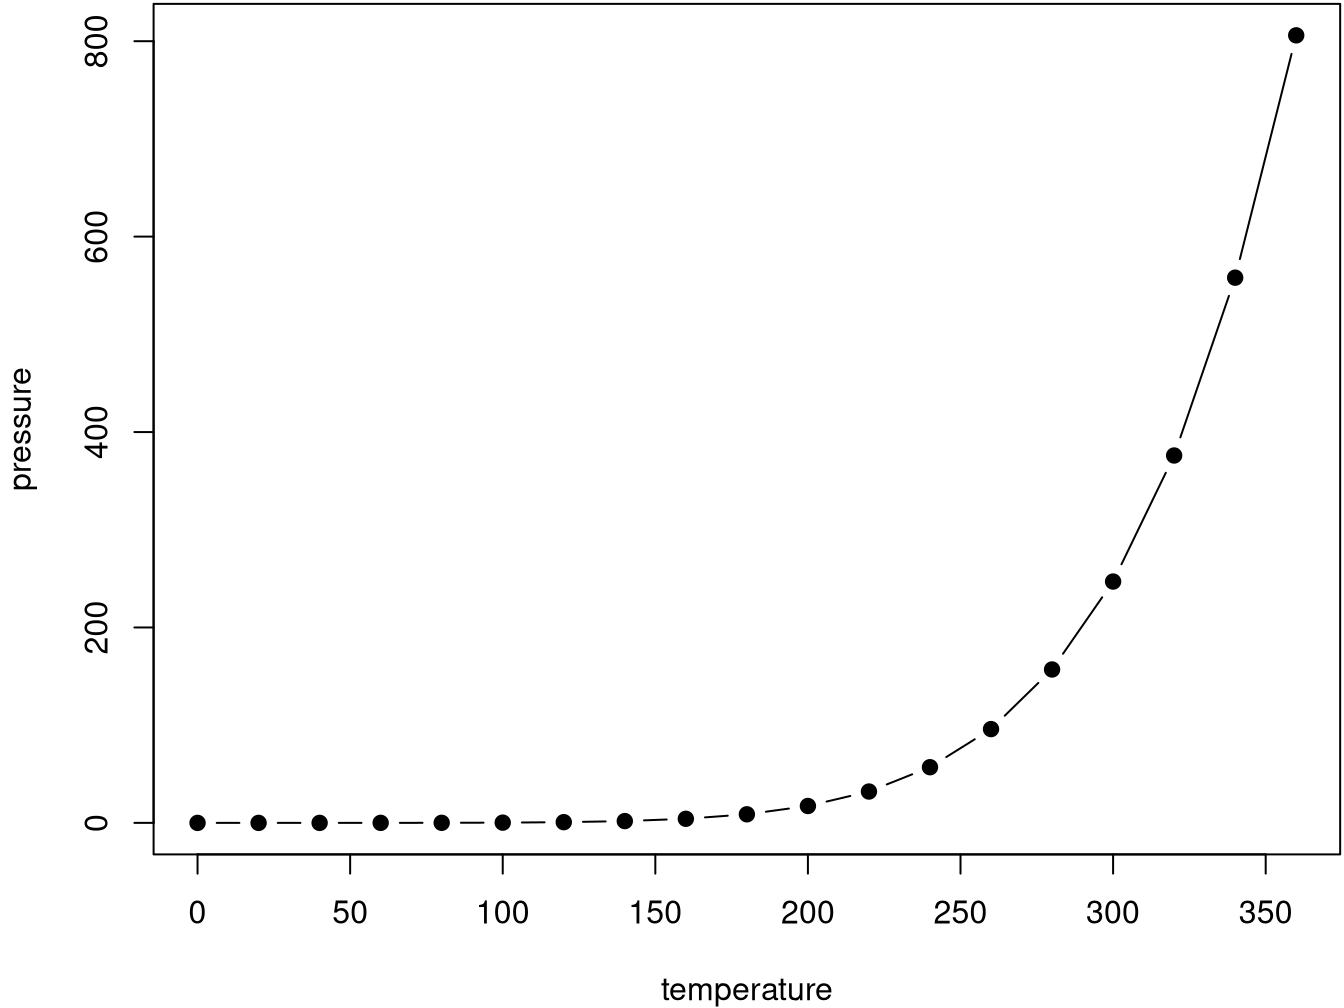
\includegraphics[width=0.8\linewidth]{Analyse-multidimensionnelle-appliquée_files/figure-latex/nice-fig-1} 

}

\caption{Here is a nice figure!}\label{fig:nice-fig}
\end{figure}

Reference a figure by its code chunk label with the \texttt{fig:} prefix, e.g., see Figure \ref{fig:nice-fig}. Similarly, you can reference tables generated from \texttt{knitr::kable()}, e.g., see Table \ref{tab:nice-tab}.

\begin{Shaded}
\begin{Highlighting}[]
\NormalTok{knitr}\OperatorTok{::}\KeywordTok{kable}\NormalTok{(}
  \KeywordTok{head}\NormalTok{(iris, }\DecValTok{20}\NormalTok{), }\DataTypeTok{caption =} \StringTok{'Here is a nice table!'}\NormalTok{,}
  \DataTypeTok{booktabs =} \OtherTok{TRUE}
\NormalTok{)}
\end{Highlighting}
\end{Shaded}

\begin{table}

\caption{\label{tab:nice-tab}Here is a nice table!}
\centering
\begin{tabular}[t]{rrrrl}
\toprule
Sepal.Length & Sepal.Width & Petal.Length & Petal.Width & Species\\
\midrule
5.1 & 3.5 & 1.4 & 0.2 & setosa\\
4.9 & 3.0 & 1.4 & 0.2 & setosa\\
4.7 & 3.2 & 1.3 & 0.2 & setosa\\
4.6 & 3.1 & 1.5 & 0.2 & setosa\\
5.0 & 3.6 & 1.4 & 0.2 & setosa\\
\addlinespace
5.4 & 3.9 & 1.7 & 0.4 & setosa\\
4.6 & 3.4 & 1.4 & 0.3 & setosa\\
5.0 & 3.4 & 1.5 & 0.2 & setosa\\
4.4 & 2.9 & 1.4 & 0.2 & setosa\\
4.9 & 3.1 & 1.5 & 0.1 & setosa\\
\addlinespace
5.4 & 3.7 & 1.5 & 0.2 & setosa\\
4.8 & 3.4 & 1.6 & 0.2 & setosa\\
4.8 & 3.0 & 1.4 & 0.1 & setosa\\
4.3 & 3.0 & 1.1 & 0.1 & setosa\\
5.8 & 4.0 & 1.2 & 0.2 & setosa\\
\addlinespace
5.7 & 4.4 & 1.5 & 0.4 & setosa\\
5.4 & 3.9 & 1.3 & 0.4 & setosa\\
5.1 & 3.5 & 1.4 & 0.3 & setosa\\
5.7 & 3.8 & 1.7 & 0.3 & setosa\\
5.1 & 3.8 & 1.5 & 0.3 & setosa\\
\bottomrule
\end{tabular}
\end{table}

You can write citations, too. For example, we are using the \textbf{bookdown} package \citep{R-bookdown} in this sample book, which was built on top of R Markdown and \textbf{knitr} \citep{xie2015}.

\backmatter
  \bibliography{book.bib,packages.bib}

\end{document}
